\documentclass{article}

\usepackage{graphicx}
\usepackage{tikz}
\usepackage{tikzsymbols}
\usetikzlibrary{calc,patterns,shapes.geometric}
\pagestyle{empty}
\usepackage[margin=0pt]{geometry}
\geometry{papersize={14in,12in}}

\def\centerarc[#1](#2)(#3:#4:#5){\draw[#1] ($(#2)+({#5*cos(#3)},{#5*sin(#3)})$) arc (#3:#4:#5);}

\begin{document}
	\begin{figure}
		\centering
		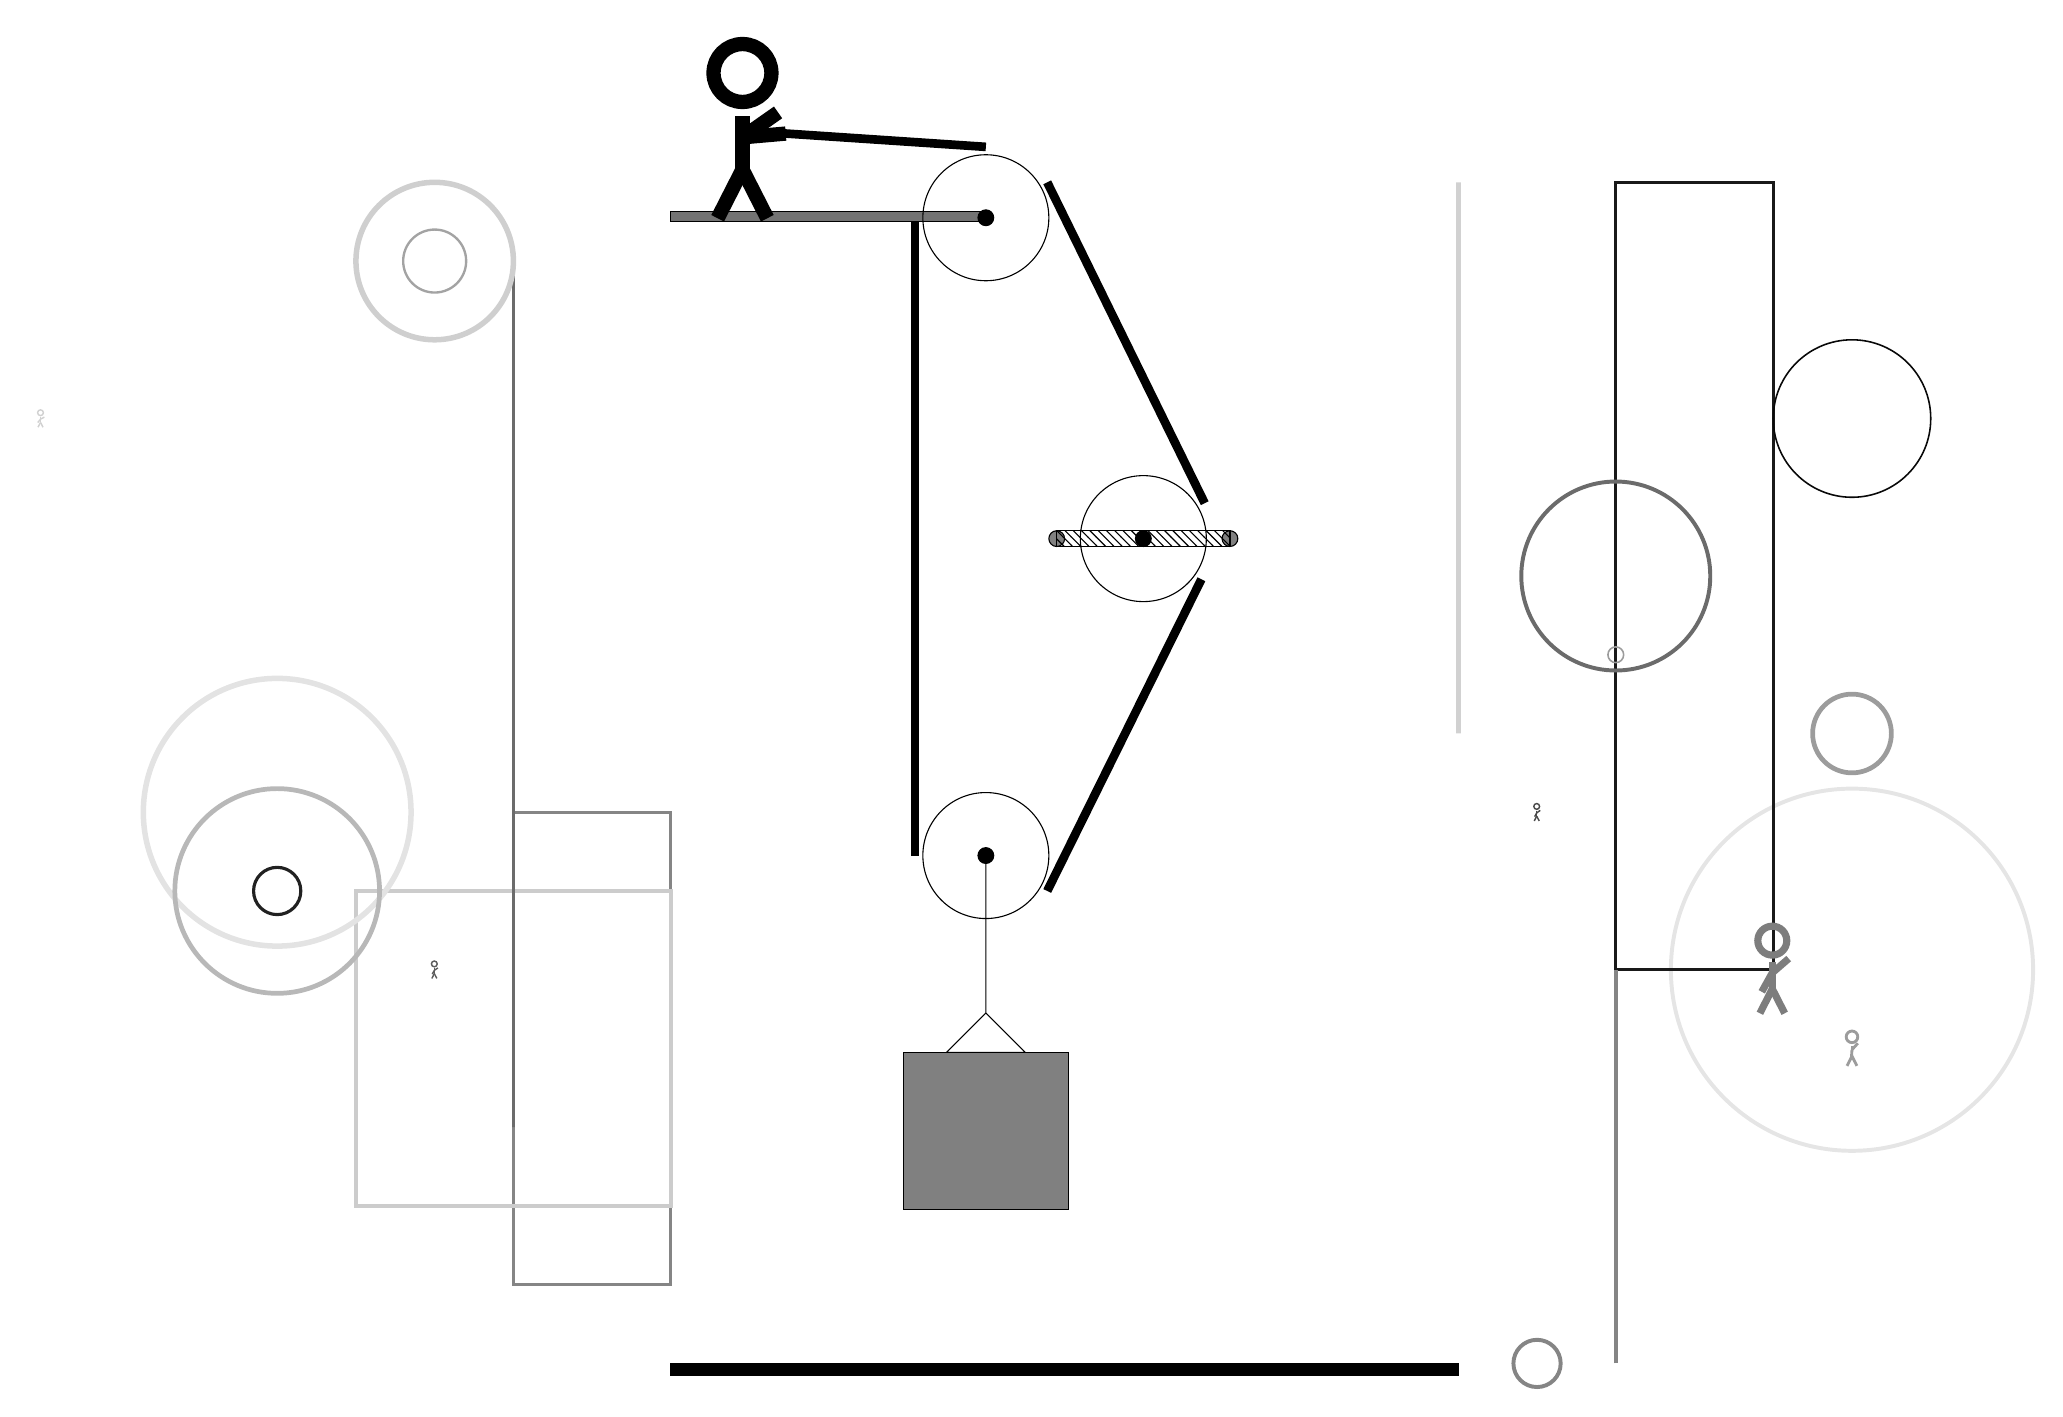
\begin{tikzpicture}
			%%%%% START %%%%%
			
			\draw[fill=black!55] (-2, 11.5) rectangle (2, 11.625);
			
			\draw (2, 3.45) circle (0.8);
			\draw[fill=black] (2, 3.45) circle (0.1);
			
			\draw [line width=0.3mm, color=black!36](-5, 11) circle (0.4);
			
			\draw [line width=0.5mm, color=black!10](13, 2) circle (2.3);
			\draw[line width=0.4mm, color=black!90] (10, 2) rectangle (12, 12);
			\draw[line width=0.4mm, color=black!48] (-4, -2) rectangle (-2, 4);
			\node[line width=0.3mm, color=black!39] at (13, 1) {\Strichmaxerl[2][86][48]};
			\draw[line width=0.5mm, color=black!20] (-2, -1) rectangle (-6, 3);
			
			\draw [line width=0.7mm, color=black!11](-7, 4) circle (1.7);
			\draw [line width=0.6mm, color=black!39](13, 5) circle (0.5);
			\node[line width=0.2mm, color=black!18] at (-10, 9) {\Strichmaxerl[1][51][28]};
			\draw [line width=0.4mm, color=black!87](-7, 3) circle (0.3);
			
			\node[line width=0.6mm, color=black!71] at (9, 4) {\Strichmaxerl[1][62][35]};
			\draw [line width=0.6mm, color=black!30](-7, 9) circle (0.0);
			\draw [line width=0.4mm, color=black!25](10, 9) circle (0.0);
			\draw[line width=0.6mm, color=black!18] (8, 12) rectangle (8, 5);
			\draw [line width=0.2mm, color=black!39](10, 6) circle (0.1);
			\draw[line width=0.4mm, color=black!58] (-4, 0) rectangle (-4, 11);
			
			\draw [line width=0.5mm, color=black!58](10, 7) circle (1.2);
			\draw[line width=0.5mm, color=black!48](10, -3) -- (10, 2);
			\draw [line width=0.2mm, color=black!97](13, 9) circle (1.0);
			\draw [line width=0.5mm, color=black!48](9, -3) circle (0.3);
			\draw [line width=0.7mm, color=black!19](-5, 11) circle (1.0);
			\node[line width=0.2mm, color=black!64] at (-5, 2) {\Strichmaxerl[1][61][34]};
			\draw [line width=0.6mm, color=black!28](-7, 3) circle (1.3);
			\node[line width=0.6mm, color=black!51] at (12, 2) {\Strichmaxerl[5][61][41]};
			
			\draw (2, 11.55) circle (0.8);
			\draw[fill=black] (2, 11.55) circle (0.1);
			
			\draw[fill=white](4, 7.475) circle (0.8);
			\draw[fill=black] (4, 7.475) circle (0.1);
			\draw[fill=black!50] (2.9, 7.475) circle (0.1);
			\draw[fill=black!50] (5.1, 7.475) circle (0.1);
			\draw[pattern=north west lines, pattern color=black] (2.9, 7.575) rectangle (5.1, 7.375);
			
			\draw (2, 3.45) -- (2, 1.45) -- (1.5, 0.95) -- (2.5, 0.95) -- (2, 1.45);
			\draw[fill=black!50] (0.95, 0.95) rectangle (3.05, -1.05);
			
			\draw[line width=1.1mm] (1.1, 11.5) -- (1.1, 3.45);
			\centerarc[line width=1.1mm](2, 3.45)(180:330:0.9);
			\draw[line width=1.1mm](2.7794, 3.0) -- (4.7373, 6.9588);
			\centerarc[line width=1.1mm](4, 7.475)(390:325:0.9);
			\draw[line width=1.1mm](4.7794, 7.925) -- (2.7794, 12.0);
			\centerarc[line width=1.1mm](2, 11.55)(30:90:0.9);
			\draw[line width=1.1mm](2, 12.45) -- (-1, 12.65);
			
			\node at (-1, 12.65) {\Strichmaxerl[10][-175][35]};
			
			\draw[fill=black] (-2, -3) rectangle (8, -3.15);
			
			%%%%% END %%%%%
		\end{tikzpicture}
	\end{figure}	
\end{document}